\section{Overview} \label{sec:overview}

\subsection{Problem Statement} \label{sec:problem}



\begin{figure*}[ht]
\begin{center}
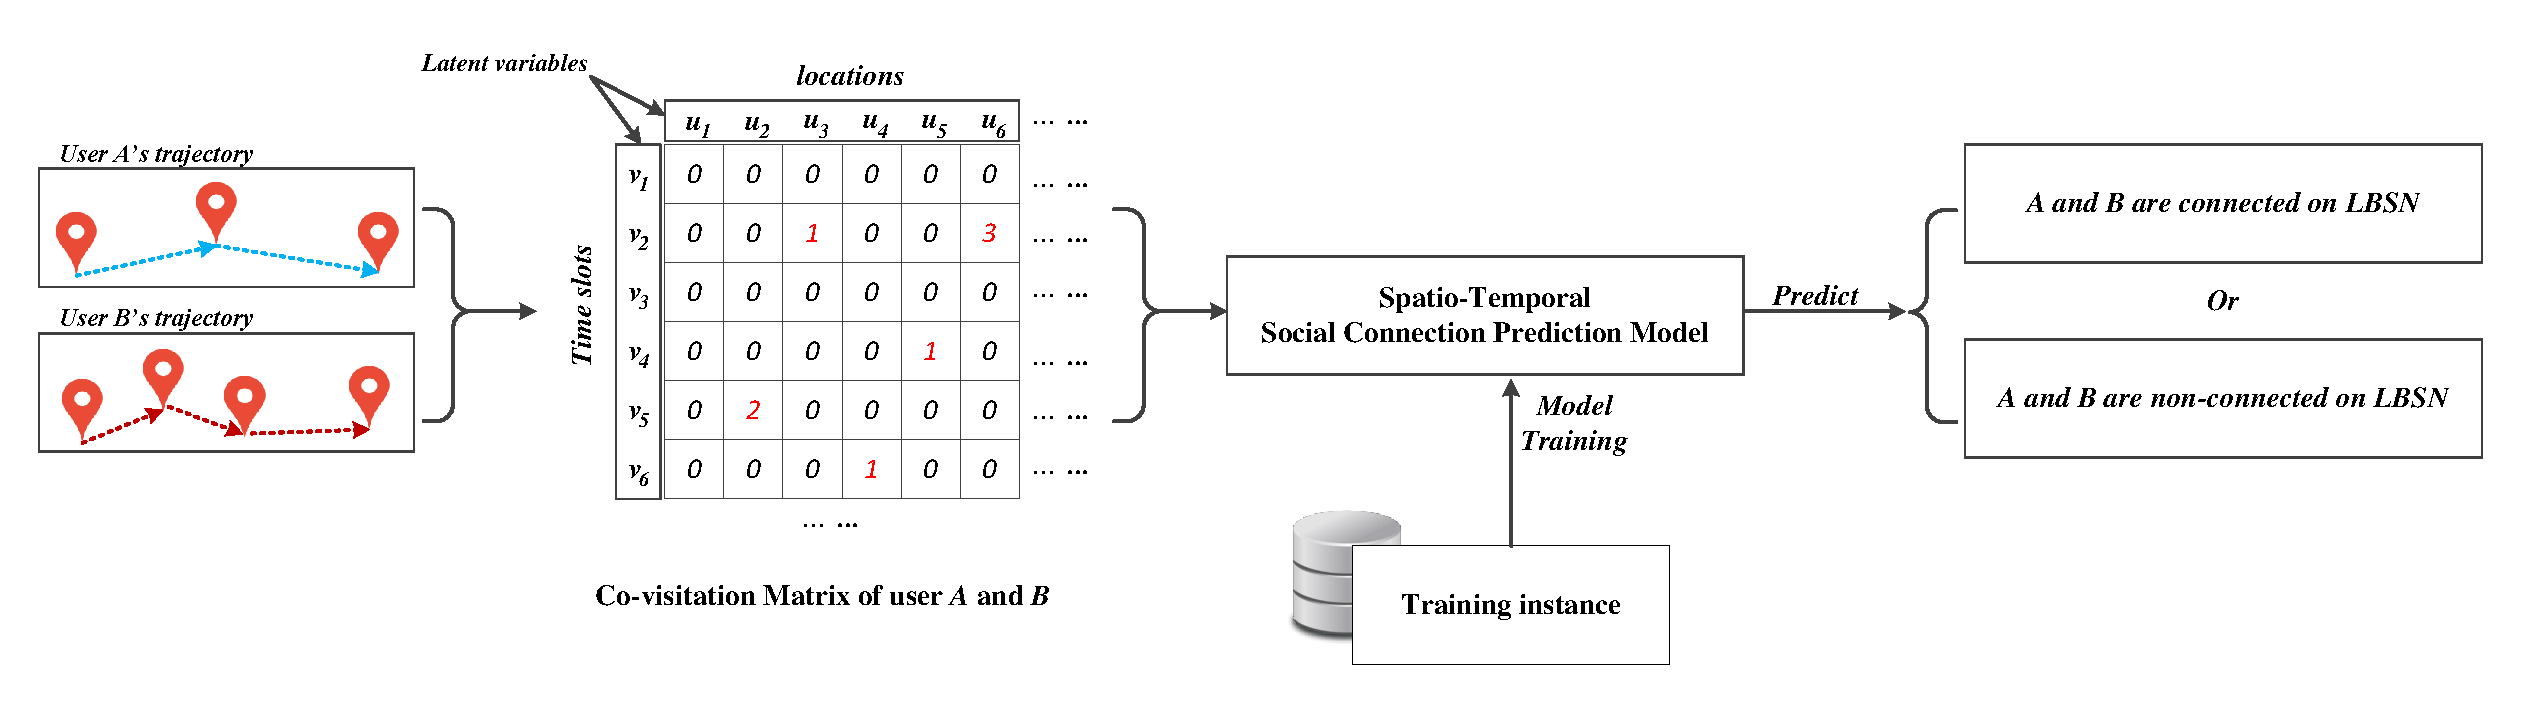
\includegraphics[scale=0.40]{steps.pdf}
\end{center}
\caption{General steps of the proposed method. }\label{steps}
%\vspace{-2mm}
\end{figure*}


We define a user's trajectory as a series of timestamped check-ins, where each check-in indicates the exact place (i.e., a restaurant, a coffee shop, etc.) the user visits, instead of a geo-graphical coordinate. The Foursquare dataset is an example of such trajectory that consists of self-reported check-ins. Note that coordinate-based trajectory can be converted into such check-ins by joining the coordinates with a database of Point-of-Interests (PoI), such as provided by Open-Stree Map. For simplicity, we consider only check-in-based trajectory in this paper. We formally define the notion of \textit{Check-in} and \textit{User Trajectory} as follows.

\begin{definition}[Check-in]
Let $\mathbb{U}$ denote a set of unique user identifiers, $\mathbb{L}$ denote a set of locations, and $\mathbb{T}$ denote the time domain. A check-in $c$ is a triple $(u, l, t) \in \mathbb{U} \times \mathbb{L} \times \mathbb{T}$, which indicates the user $u$ has visited $l$ at time $t$.
\end{definition}

\begin{definition}[User-trajectory]
Let $\mathbb{C}$ be a collection of check-ins and $u \in \mathbb{U}$ a user, then the set $C_u := \{ (u', l, t) \in \mathbb{C} | u = u'\}$ is the user-trajectory (or simply trajectory) of $u$.
\end{definition}

The proposed social connection prediction model is based on the concept of \textit{Co-visitation}, which is defined as follows: 

\begin{definition}[Co-visitation]
A co-visitation of two users $u_i$ and $u_j$ to a location $l$ is defined as the event that $u_i$ and $u_j$ report two check-ins $(u_i, l, t_i)$ and $(u_j, l, t_j)$ respectively, where $| t_i - t_j| \leq \tau$.
\end{definition}

Here $\tau$ is an experience-based parameter called the co-visitation time window. We formulate the social connection prediction problem as a classification problem. Given the trajectory of two users $u_i$ and $u_j$, the goal is to assign the pair of users $(u_i, u_j)$ into one of the two classes: \textit{Connected} or \textit{Not-connected}.

Note that the above problem formulation implicitly assumes the social connection is mutual, i.e., if $u_i$ is a friend of $u_j$, then $u_j$ is also a friend of $u_i$. This type of social connection is common on most LBSN like Facebook. For such connections, the class of a pair of users is not order sensitive. However, on some LBSN the social connection can be one-way. For example, on Foursquare, a user can choose to ``follow" other users and thus formulates a one-way social connection, where one user is the \textit{follower} and the other being the \textit{followee}. The one-way social connection can be model by treating $(u_i, u_j)$ and $(u_j, u_i)$ as different instance which can be assigned into different classes.


\subsection{Methodology} \label{sec:method}

We model the probability of the existence of social connection between two users based on the hypothesis that socially connected users tend to visit same locations at same time periods, which is defined as co-visitations. However, we observes that in reality not all co-visitations are equally important in terms of predicting user's social connections. We propose a three step model learning process to capture this difference (Figure~\ref{steps}).

\begin{itemize}
\item \textbf{Co-visitation Matrix formulation} Given the trajectories of two users $u_i$ and $u_j$, we first convert their trajectories into a spatio-temporal co-visitation matrix that records the time and location of their co-visitations.

\item \textbf{Probability estimation}  The probability that $u_i$ and $u_j$ are socially connected is computed based on their co-visitation matrix.

\item \textbf{Model learning} The latent variables in the model are estimated by optimization a loss function, which measures the prediction error between actual class and predicted class for each pair of users in the training set.
\end{itemize}

We present details of these three steps in the next section.

\iffalse

Research questions worth exploring in the future

1. Active user vs Non-active users?
2. Percentage of social connections can be explained by trajectories? 
3. Most significant types of locations?
4. Most significant time slots?
5. Geo-distance and predictive power?

\fi